\documentclass[a4paper]{article}

\usepackage[english]{babel}
\usepackage[utf8x]{inputenc}
\usepackage{amsmath}
\usepackage{graphicx}
\usepackage[colorinlistoftodos]{todonotes}

\title{Advanced Monte Carlo of the Two-Dimensional Ising Model}
\author{Brandon Ewert}

\begin{document}
\maketitle

\begin{abstract}
We revisit the simulation of our magnetized lattice with periodic boundary conditions. This project, however, relies on an entirely different algorithm to update the lattice over time. Rather than flip individual spins based on Boltzmann factor probabilities at each increment of time, we grow clusters of flipped regions. Our working algorithm, dubbed the Wolff Algorithm, more accurately predicts the critical temperature at which the magnetization of the lattice abruptly decays to zero. With the help of some clever queuing, the Wolff Algorithm is simple to implement and produces very neat results. Python was chosen for its readability and simplicity, regardless of its sluggishness. 
\end{abstract}

\section{Introduction}


Our goal is to characterize the lattice’s internal energy, magnetization, magnetic susceptibility, and heat capacity as functions of absolute temperature. The moving parts of this project are the individual spins that comprise the lattice. A lattice site has two states – ‘up’ or ‘down’, and are denoted by a +1, -1, respectively. Generally, spins are able to flip states based on a probability derived from statistical mechanics. We simulate the change of this magnetization over time by sampling the lattice’s magnetization and energy many times. This sampling according to probability is dubbed a Monte Carlo Simulation, and was first devised to estimate the critical mass of uranium needed to ignite a fission chain reaction in the world’s first atomic bombs. 


Slightly more benevolently, we use this process to calculate internal energies and total magnetizations of our lattice after the flipping spins of the lattice has reached equilibrium at a given temperature. Figure 1 shows the equilibration of magnetization at high temperatures. Due to the nature of our flipping algorithm, significantly more time is needed for higher temperature lattices to equilibrate than for low temperatures (T < 3). We do this iteratively for many temperatures to produce clean data and simulate the demagnetization of a magnetized object. It is well known that higher temperatures, magnetic domains tend to orient themselves randomly do to thermal jostling – an aspect characterized by the Critical Curie Temperature of a material. This temperature is one beyond which a material will have net magnetization zero given no external magnetic field. It is where the derivative of magnetization with respect to temperature is maximized. Figure 2 illustrates the Critical Curie Temperature of a lattice. The data is noisy, since it was not averaged over multiple iterations. We expect the internal energy of the sample to follow the same suite – a quick die-off near the critical temperature and smoothing out near at extreme temperatures. Heat capacity and magnetic susceptibility are derivatives of these functions with respect to temperature, and will therefore be very simple to calculate numerically. 


\section{Implementation}



We start our simulation by constructing a lattice of homogeneous spin (we choose spin up, with value+1). A Python list of lists works nicely – one list encapsulates individual lists for each row. Each row list contains the spins themselves. For simplicity, we choose a square lattice (the number of rows is the number of spins in each row). The function $Lattice Initializer$ takes dimension as an input and returns a full list that will serve as our lattice. Our methods of sampling goes as follows:


	1.	We choose a random site in the lattice, whose spin is immediately flipped


	2.	We approximate the effect of this spin flip to influence only the four nearest neighbors (up, down, left, right)


	3.	The contribution to the total internal energy of the original site is calculated 

 	
	4.	Based on individual probabilities, we flip the neighbors’ spins

 
	5.	Step 2 is repeated at each of the flipped neighbors, until a cluster of flipped spins is built


	6.	The cluster stops expanding if either the probability limits its advance, or all sites have been flipped

 
	7.	We grow another cluster and iterate this process until the lattice reaches an equilibrium spin state

 
	8.	The magnetization is calculated by adding up individual site spins at equilibrium

 
This process is known as the Wolff Algorithm, and, though implementation can prove to be quirky, it is a more accurate simulation of demagnetization than the Metropolis Algorithm. The Metropolis test is identically the first four steps of the Wolff Algorithm, iterated continually until equilibrium is met. The advantage of building clusters is that it allows spins to effectively communicate with other parts of the lattice, rather than just nearest neighbors. Magnetic fields from individual spins are small, but limiting their range to nearest neighbors weakens the lattice’s ability to demagnetize quickly, and provide accurate data around the critical temperature.


Choosing a random site is simple enough. An integer between zero and one less than the dimension squared is generated by Python’s built-in Random library. The modulo of this number and the dimension is the column number (starting with zero), and the row number is the remainder of the random integer and the dimension. 

To check the site’s neighbors, we add and subtract one to both the column and row numbers of the site. Python’s lists are backward periodic, meaning a negative list index starts counting from the end of the list back toward the front. This allows us to easily apply periodic boundary conditions. That is, spins on boundaries of the lattice those on the opposite side. Periodicity is a clever way to simulate an infinite lattice, as if we are only looking at a small sample of a much larger material. Adding one to a boundary column or row number (up, right neighbors) will produce an index that is inaccessible on a Python list. For this reason, we use modulo division to catch those overrunning indices and set them back to the beginning of the list.  To avoid complications with negative list indices (left, down neighbors), we use a conditional to sort whether a list index is a boundary or inner site. See the function $Cluster NN$ for further detail.


Internal energy is calculated by summing over all interactions between spins in the lattice. Here, we limit our concern to nearest neighbors, condensing our sum to four terms at each individual site. Our lattice begins in its lowest energy state – all spins are aligned. With thermal vibrations at increasing temperature, the energy is expected to increase to nearly zero (if the number of spins up is exactly the number of spins down). We start each iteration of the algorithm by setting the energy equal to zero, and simply adding contributions dynamically until clusters have ceased growing. The final energy is the total for the lattice. 

$$E = \sum_{i,j}^{N} S_i S_j$$


The probability component of the algorithm is one that satisfies detailed balance – a particular situation in which the probability current within our statistical sum is conserved. At the end of the day, whether or not a site will flip can be determined by random number generator compared to a Boltzmann-esque factor. We choose a random number between zero and one, and if it is less than the factor, the neighboring spin will flip. Note that at higher temperatures, the exponential approaches one, meaning spins will rarely flip. Conversely, low temperatures ensure spins flip at almost every time. 


We do expect, however, that high temperatures will yield low magnetizations. How then, do we justify the disparity between cluster size and magnetization? As Connor would blurt; “Equilibrium!”  At high temperatures, our clusters may only consist of a few sites. We must grow many clusters at high temperatures to reach equilibrium, where magnetization no longer changes over time. At low temperatures, we need only to grow one or two clusters to ensure equilibrium is reached. The “time” we run our algorithm (or, rather, the number of clusters we grow), should scale with temperature. We could just find the number of clusters that yield good results for high temperatures, but this needlessly draws out our low – temperature calculations. Since the clusters nearly encapsulate the entire lattice at low temperatures, our data would take drastically longer to compute. To simplify our data, we choose the Boltzmann constant and coupling constant of spin interactions to both be one. This yields unitless results for all values. Our temperature range, arbitrarily, is set between 1 and 3.5. From previous tests, we have deduced the critical temperature to be around T = 2.3 . Our number of clusters grown for different temperatures has been empirically tried and tested. Here I quote the results, contained within the function $Temp  Run$. 


	1. For T greater than 1.7 , the 8 clusters suffice to meet equilibrium
    
  
	2. For  T between 1.7 and 1.9, we bump up the number to 45
    
    
	3. For T between 1.9 and 2.5, we ramp the number of clusters to the dimension squared
    
   
	4. For all higher temperatures, the number stays constant at twice the dimension squared
    
 
Now, having chosen our neighbors that are to be flipped, we look at the neighbors or those neighbors – and so on. One efficient way of keeping track of this increasingly large array of neighbors is to apply a queuing algorithm. In Python, lists also serve as a decent queue. Every time we decide a neighbor is slated to flip, we store it in the queue, where it can later be dealt with. To prevent us from adding the same neighbors infinitely, we change the sign of the spin before a neighbor is added to the queue, and add a stipulation that flipped spins are not allowed in the queue. This way, we only flip ones to negative ones, and never the other way around (unless the randomly chosen site lands on a site that was a previously flipped neighbor or chosen site). We store information in the queue as a list of spin, column and row. Once the queue has been completed (the cluster growth halts), we can iterate through it. The queue will initially only contain up to four neighbors from the first site. This initial queue is set up in the function… drum roll please!... $Initial   Queue$. We ‘pop’ the first neighbor, which removes it from the queue, and we look at its neighbors. This potentially adds another set of sites to the queue, and we proceed until the queue is void of sites. This is done for different numbers of clusters, as prescribed above. 


The magnetization of the lattice is calculated by iterating through the lattice list and adding spins. It is expected that at low temperatures, we may reach negative magnetizations. Not only does this happen, but at very low temperatures, the signs of the magnetization oscillates from negative to positive. This is because we start with a homogeneous positive magnetization, which will almost entirely flip to all to negative. If we build another cluster, we flip the whole lattice from negative to positive again. We plan on running the simulation many times to average out data, so this oscillation can prove problematic. For this reason, we take the absolute value of the magnetization at lower temperatures (T less than 2.5), and for higher temperatures, the magnetization is allowed to be negative or positive to average out to clean values. 


To plot the energy and magnetization versus temperature, we iterate the same process through a range of temperatures. At each temperature, we run the simulation until the lattice has equilibrated, nab the energy and calculate the magnetization, and append it to a list. The list contains these values for the full range of temperatures (again, from 1 to 3.5, and in steps of .007). We do this several times and average the data, and calculate error bars. Mathematica is used because of its efficiency and convenient drawing tools. 
For the plots of magnetic susceptibility and heat capacity, we take numerical derivatives of the magnetization and internal energy, respectively. Since temperature is unitless, our numerical derivative is very simple. 

$$\frac{df}{dx} = f(x+1) - f(x) $$

\section{Results}

All graphs are of 100x100 lattices, averaged over 10 runs. More runs smooth the data considerably. 

\subsection{Magnetization}

We report a very smooth taper until the critical temperature, where the slope approaches infinity. Figure 3 depicts the magnetization as a function of temperature. We notice a smoothing down of the magnetization directly after the critical temperature. This suggests that we could have grown more clusters in this region for a sharper descent.

\subsection{Magnetic Susceptibility}

Despite the noise, it is clear that our Curie Temperature lies between 2.4 and 2.5 (the graph is on the interval [1,3.5] in steps of .01). This is very close to the accepted value of 2.26. Note that the noise is amplified for temperatures above the Curie point. More averaging would certainly help tame the fluctuating trail at higher temperatures.

\subsection{Internal Energy}

Remarkably smoother than our magnetization graph, we see the energy die off (or, rather, increase from zero, since the internal energy is negative for low energy states) as the magnetization does. The scale is unnormalized, but it does a good job of showing its temperature lag. The magnetization seems to die off about .5 units before the energy. We expect a curved trajectory to zero at the Curie Temperature.

\subsection{Heat Capacity}

A bit more symmetric, this graph indicates a clear rise centered just past the Curie point, at about T = 2.8. We expect to see a sharp rise to its maximal value at the Curie point, and a discontinuous trail to zero past this temperature. The outliers in the center region obscure its  true shape, but the graph captures the Heat Capacity's general trend. 

\section{Summary}

Our algorithm produces decent data, but could certainly use a speed boost. Generating the 10-iteration plots takes nearly 6 hours without optimization. There is room to improve with the coding efficiency, and with the smoothness of our graphs. Given a more powerful computer, we would be able to generate much neater curves yet larger lattices. Our method, though is fairly accurate at plotting the trends of magnetization and energy with temperature. 



\begin{figure}
\centering
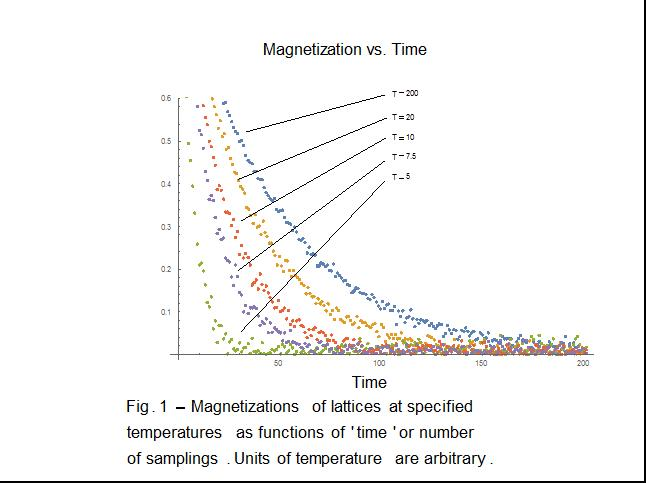
\includegraphics[width = 15cm]{M.jpg}
\end{figure}

\begin{figure}
\centering
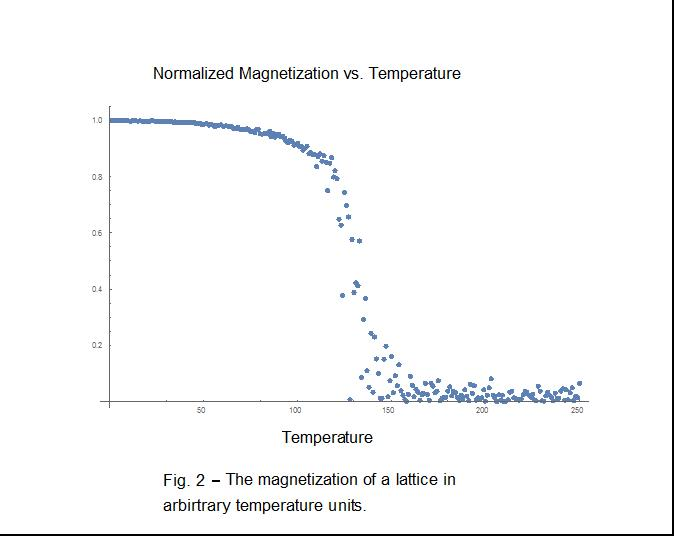
\includegraphics[width = 15cm]{Mag_v_Temp_single_iter.jpg}
\end{figure}

\begin{figure}
\centering
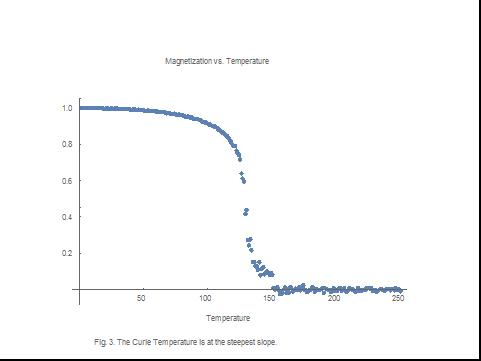
\includegraphics[width = 15cm]{fig4.jpg}
\end{figure}


\begin{figure}
\centering
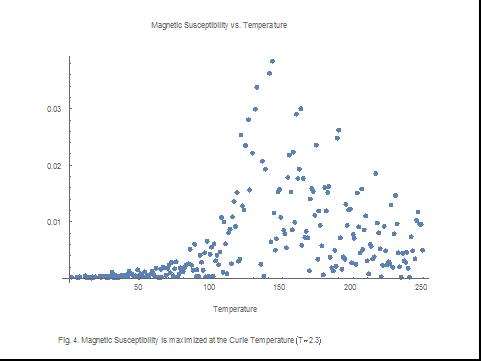
\includegraphics[width = 15cm]{fig3.jpg}
\end{figure}


\begin{figure}
\centering
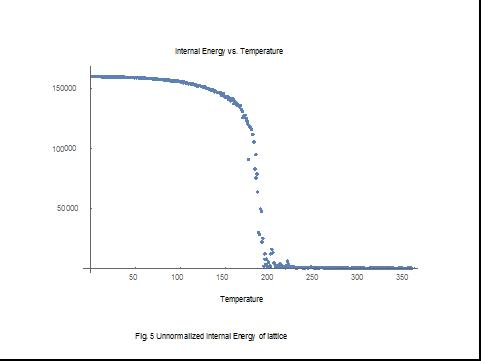
\includegraphics[width = 15cm]{fig5.jpg}
\end{figure}


\begin{figure}
\centering
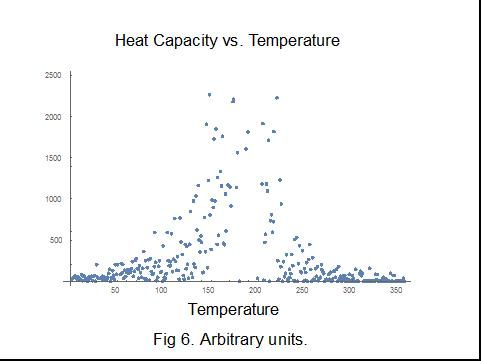
\includegraphics[width = 15cm]{fig6.jpg}
\end{figure}
\end{document}